\documentclass{article}%
\usepackage[T1]{fontenc}%
\usepackage[utf8]{inputenc}%
\usepackage{lmodern}%
\usepackage{booktabs}%
\usepackage{textcomp}%
\usepackage{lastpage}%
\usepackage{geometry}%
\usepackage{amsmath}%
\geometry{
    paper=a4paper,
    head=0cm,
    left=2cm,
    right=2cm,
    top=0cm,
    bottom=2cm,
    includehead=True,
    includefoot=True
}%
\usepackage{graphicx}%
%
\usepackage{multicol}%
\usepackage{lipsum}%
\usepackage{float}%
\usepackage{verbatim}%
\title{
    Reconstructing Arrival-Times of individual Night-Sky-Photons using many small Photo-Sensors and slow Read-Out.
}%
\author{Sebastian A. Mueller, Thomas Kihm, and Werner Hofmann}%
\date{\today{}}%
%
\begin{document}%
\maketitle%

\newcommand{\F}{F_\text{nsb}}
\newcommand{\Ftyp}{F_\text{typical}}
\newcommand{\Apulse}{A_\text{pulse}}
\newcommand{\fadc}{f_\text{adc}}
\newcommand{\fproc}{f_\text{proc}}

\begin{multicols}{2}%
%
The atmospheric Cherenkov-method can reconstruct the type, energy, and direction of a cosmic particle from an air-shower's Cherenkov-light.
%
Cherenkov-telescopes sense blueish Cherenkov-light, better reject reddish night-sky-light, and reconstruct the arrival-times of photons with $\sim{}$5\,ns resolution.
%
Photo-sensors and read-out are cost-drivers of the method.
\newline
%
We expect a continues read-out into digital buffers, where each individual photon is recorded, to be beneficial for the atmospheric Cherenkov-method as it allows fast computational access to all observables.
%
The energy-threshold can be lower \cite{jung2005star}, the separation of Cherenkov- from night-sky-light can be better, and overall the reconstruction of the cosmic particle will benefit\cite{catalano2008single}.
\newline
%
One way of continues read-out are flash analog-digital-converters (ADC)s.
%
However, their cost and power-consumption scale rapidly with their sampling frequency $\fadc{}$.
%
\begin{eqnarray*}
\text{Cost} &\sim& \fadc{}^2,\\
\text{Power} &\sim& \fadc{}^2.
\end{eqnarray*}
%
In this report, we explore a read-out with many slow \mbox{($f$ < 100\,MHz)} ADCs.
%
We want each ADC to digitize the signal of a photo-sensor that has little acceptances (area $\times{}$ solid angle) and thus a low rate of night-sky-photons.
%
We hope that when the rate of night-sky-photons is low, a slow ADC and a little computing will be able to reconstruct the arrival-times of the individual photons sufficiently accurate with $\pm5\,$ns, i.e. better than the sampling-period $1/\fadc{}$.
%
Since the cost of silicon photo-sensors are mostly proportional to their area, there is only little overhead when replacing a big sensor with multiple small ones.
%
Due to the rapid scaling of the ADC's demands with sampling-frequency $\fadc{}$, many slow ADCs might outperform fewer fast ADCs in both power-consumption and cost.
\newline
Further, the finer binning of photo-sensors might allow plenoscopes with large  field-of-views ($> 300\,(1^\circ{})^2$) due to computational compensation of optical aberrations. \cite{mueller2019phd}.
%
\section*{Sensing Night-Sky-Photons}%
\label{sec:nsb}%
%
Table \ref{TabFilters} shows the relative yield $\eta_\text{Cer.}$ of Cherenkov-light, and the resulting rate $R_\text{nsb}$ of night-sky-photons for typical photo-sensors.
%
\begin{table}[H]
  \begin{center}
    \begin{tabular}{cccrr}
%
        \footnotesize{sensor} &
        \footnotesize{mirror} &
        \footnotesize{filter} &
        $R_\text{nsb}$ /   &
        $\eta_\text{Cer.}$ / \\
%
        &
        &
        &
        \footnotesize{$10^6\,\text{m}^{-2}\,(1^\circ)^{-2}\,\text{s}^{-1}$} &
        \footnotesize{$10^{-3}$} \\
%
        \hline
        PMT &             &             & 144.8 & 213\\
        .   & $\bullet{}$ &             & 135.8 & 206\\
        .   & $\bullet{}$ & $\bullet{}$ &  15.9 &  53\\
        \hline
        SiPM &             &             & 280.3 & 198\\
        .    & $\bullet{}$ &             & 188.5 & 176\\
        .    & $\bullet{}$ & $\bullet{}$ &   7.1 &  24\\
    \end{tabular}
    \caption{
The rates and yields result out of the typical flux of night-sky-light $\Ftyp{}$, see Figure \ref{fig:nsb}, the sensors detection-efficiencies, see Figure \ref{fig:pde}, and the efficiencies of a  mirror and a filter, see Figure \ref{FigNsbFilter}.
    }
    \label{TabFilters}
  \end{center}
\end{table}
%
The typical flux of night-sky-light corresponds to a sky surface brightness of
%
\begin{eqnarray*}
\Ftyp{} &\hat{=}& 21\,\text{mag}\,\text{arcsec}^{-2}.
\end{eqnarray*}
%
Most observations take place in the range of fluxes from
\begin{eqnarray*}
\approx{}0.8 &> \F{} / \Ftyp{} >& \approx{}4.
\end{eqnarray*}
%
Figure \ref{fig:obstimeFact} shows the distribution of $\F{}$ for a Cherenkov-telescope that deliberately pushed observations into the brightest full moon conditions.
%
Even then, observations beyond $\F{} / \Ftyp{} = 5$ are rare.
%
Table \ref{TabInstrumentsNsbRates} shows the expected rates of night-sky-photons in different instruments.
%
\begin{figure}[H]%
\centering%
\includegraphics[width=1.0\linewidth]{night_sky_background.jpg}%
\caption{
The typical flux $F_\text{Night}$ of night-sky-light \cite{gaug2013night}.
Dotted line is \cite{preuss2002study}.
Gray line is a simulated and arbitrarily scaled Cherenkov-spectrum of a 5\,GeV gamma-ray in Chile at 5\,km a.s.l.
All extrapolated from 700 - 1000\,nm.
}%
\label{fig:nsb}
\end{figure}
%
\begin{figure}[H]%
\centering%
\includegraphics[width=1.0\linewidth]{photon_efficiency.jpg}%
\caption{
Dashed line is silicon-photo-multiplier (SiPM), \mbox{Hamamatsu\,S10362-33-050C}, shape according to \cite{hamamatsu2009mppc}, and scaling according to \cite{anderhub2013design}.
Extrapolated from 700 - 1000\,nm.
Dotted line is photo-multiplier-tube (PMT), \mbox{Hamamatsu\,R11920-100-05} \cite{toyama2013novel}
}%
\label{fig:pde}
\end{figure}
%
\begin{figure}[H]%
\centering%
\includegraphics[width=1.0\linewidth]{nsb_filters.jpg}%
\caption{
Dashed line is CTA's dielectric mirror for the MST, after degrading \cite{pareschi2013status,pareschi2013statusarxiv}.
%
Dotted line is VERITAS' night-sky-filter \cite{archambault2017gamma}.
%
Both Extrapolated from 700\,nm to 1000\,nm.
}%
\label{FigNsbFilter}
\end{figure}
%
\begin{figure}[H]%
\centering%
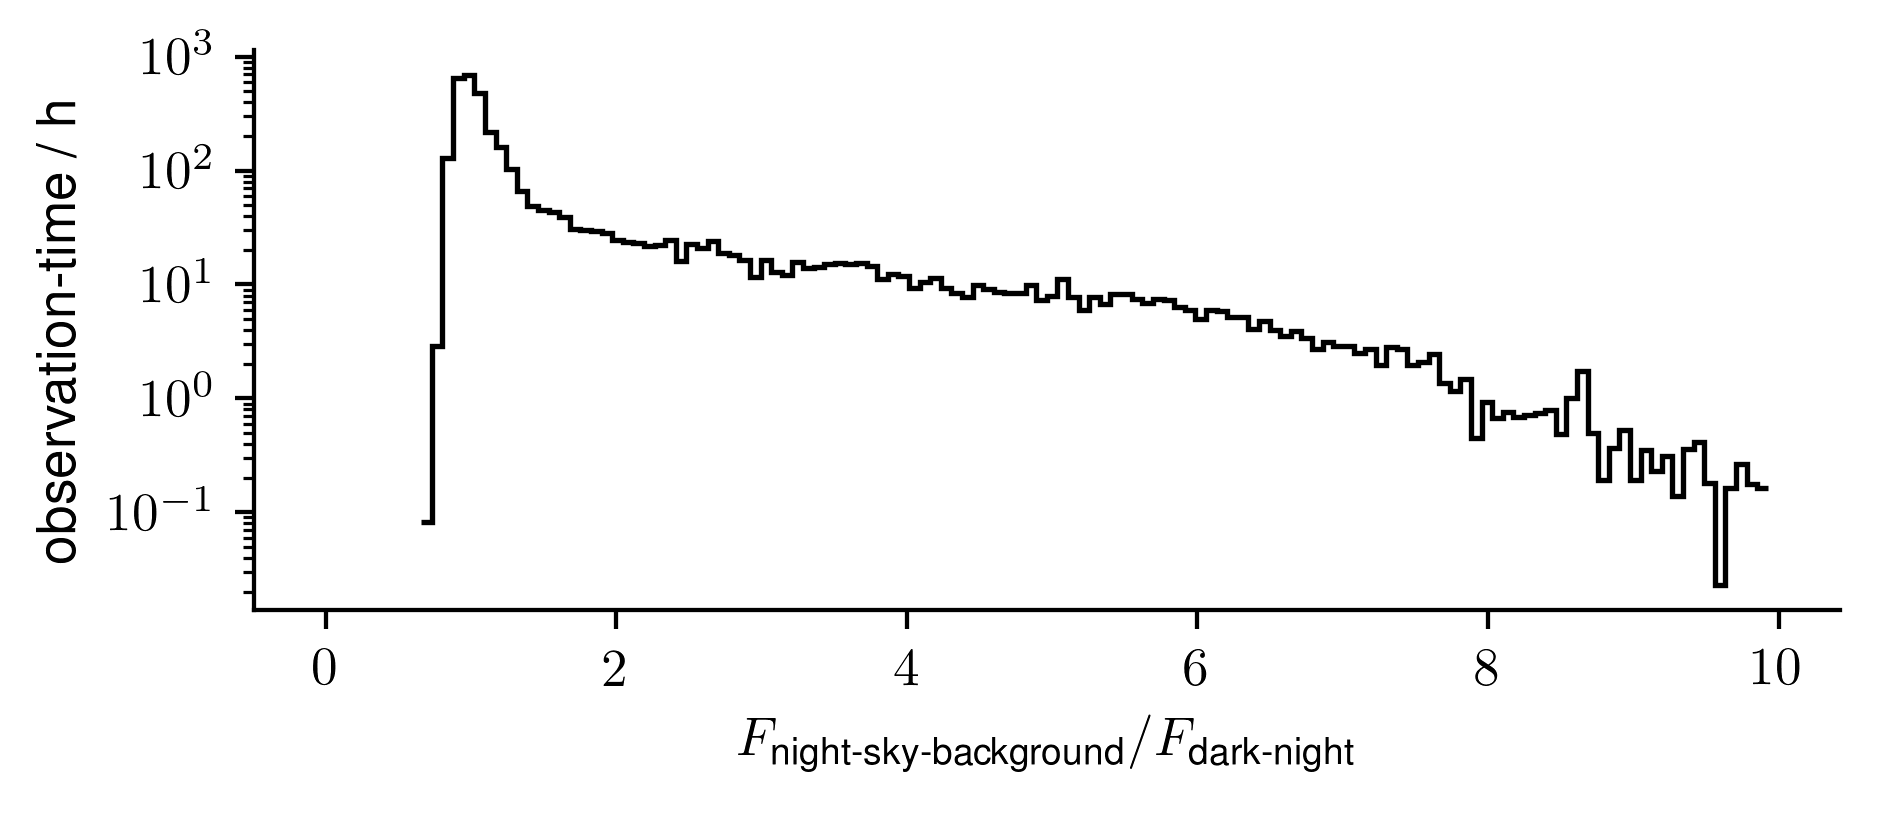
\includegraphics[width=1.0\linewidth]{observation_time_histogram.png}%
\caption{
Figure taken from \cite{mueller2019phd}.
%
The distribution of FACT's observation-time vs. the flux of night-sky-light.
}%
\label{fig:obstimeFact}
\end{figure}
%
\begin{table}[H]
  \begin{center}
    \begin{tabular}{lcrrr}
        &tech.& area/ & fov/&$R_\text{nsb}$/\\
        &     & m$^2$ & $(1^\circ)^{2}$&$10^6$s$^{-1}$\\
      \hline
      FACT &SiPM& 10 & 0.01 & 29\\
      H.E.S.S. CT-1 &PMT& 108 & 0.0222 & 344\\
      H.E.S.S. CT-5 &PMT& 614 & 0.0039 & 347\\
      Portal, 71m &PMT& 65 & 0.0039 & 37\\
    \end{tabular}
    \caption{Expected rates of night-sky-photons $R$ in an individual read-out-channel (pixel or lixel).}
    \label{TabInstrumentsNsbRates}
  \end{center}
\end{table}
%
\section*{Simulating a slow ADC-read-out}%
\label{SecSimulating}%
%
To estimate the reconstruction power of a read-out with slow sampling ADC's, we run a simulation.
%
We simulate the electric response of a silicon photo-sensor (G-APD-array).
%
Our readout is designed around an ADC with a sampling-rate $\fadc{}=83.3$\,MHz and a resolution of 8\,bit.
%
Table \ref{TabReadOutConfig} shows the configuration of our read-out.
%
\begin{table}[H]
    \begin{center}
        \begin{tabular}{lr}
            Analog path & \\
            \hline
            low-pass' cut-off & $\fadc{}/2 = 41.7$\,MHz\\
            &\\
            Pulse & \\
            \hline
            decay-time mean & $50$\,ns\\
            decay-time std. dev. & $1$\,ns\\
            amplitude mean & 1.00\\
            amplitude std. dev. & 0.01\\
            amplitude low-pass $\Apulse{}$ & 0.81\\
            &\\
            ADC & \\
            \hline
            sampling-frequency $\fadc{}$ &$83.3$\,MHz\\
            noise-amplitude & $0.1\Apulse{} = 0.08$\\
            amplitude min. & $-0.8\Apulse{} = -0.65$\\
            amplitude max. & $+12.0\Apulse{} = +9.83$\\
            resolution & 8\,bit\\
            &\\
            Processing & \\
            \hline
            sampling-frequency $\fproc{}$& $6\fadc{} = 500.0$\,MHz\\
            resolution & 10\,bit\\
        \end{tabular}
        \caption{%
The configuration of the simulated read-out. The spread of decay-times and amplitudes for the pulse are taken from the author's experience with the SiPMs and gain-feedback of FACT, and are negligible. See also \cite{fact-performance}.
}
        \label{TabReadOutConfig}
    \end{center}
\end{table}
%
\subsection*{Analog path}%
%
The analog path of our read-out is designed to match $\fadc{}$ with a gain that drops down to 1/2 (-3dB) at the ADC's Nyquist-frequency $f = \fadc{}/2$, see Figure \ref{FigSimAnalogTransmission}.
%
The electric coupling to the photo-sensor is chosen for the pulse to have a decay-time that covers multiple ADC samples.
%
To avoid additional noise and artifacts, we do not use pulse-shaping such as $\lambda /2$ reflections.
%
Figure \ref{FigSimPulseTemplate} shows our electric pulse in the analog path and Figure \ref{FigSimPulsePhases} shows the pulse for various relative phases w.r.t. the ADC's sampling.
%
\subsection*{ADC}%
%
Our ADC has a white noise-amplitude of $0.1\Apulse{}$ \footnote{The same noise-amplitude as FACT.}, where $\Apulse{}$ is the maximum amplitude of the pulse at the ADC's input, i.e. after the low-pass.
%
Our ADC's amplitude-range spans from $-0.8\Apulse{}$ to $12.0\Apulse{}$. This means it will saturate for a coincident stack larger than 12 photons and gives us about 20 amplitude-steps for $\Apulse{}$.
%
\subsection*{Processing path}%
%
Our digital processing over samples the ADC's signal with a sampling-frequency of $\fproc{} = 6\fadc{} = 500.0$\,MHz, and with a four times higher amplitude-resolution of 10\,bit.
%
The digital processing does not interpolate or smooth the ADC's signal, but for example in internal convolutions with a kernel-function the processing makes use of its higher resolution.
%
We design all algorithms for the digital processing without conditional branching, i.e. easy to implement with basic logic gates.
%
We have Field-Programmable Gate Arrays (FPGA)s in mind, but happily use CPUs when fast enough.
%
\subsection*{Extracting photon-arrivals}%
%
We test two algorithms to extract the arrival-times of photons from the digital signal.
%
These algorithms run in the digital processing path of our read-out and thus operate with sampling-frequency $\fproc{}$ and 10\,bit amplitude-resolution.
%
They are FPGA-aware.
%
\subsubsection*{Convolution-Maximum}%
%
Our first algorithm convolves the signal with a template of the pulse's rising edge, see Figure \ref{FigSimRisingEdgeTemplate}.
%
When the response of the convolution is above a threshold of $0.4\Apulse{}$, AND when the gradient of the response is rising, AND when all these conditions where not in the previous time-sample, than the current time-sample is identified to be the arrival of a pulse.
%
\subsubsection*{Multi-Subtraction}%
%
The second algorithm also convolves the signal with the template of the pulse's rising edge. It also uses the response of the convolution to estimate the arrival-time of a pulse.
%
But it does not take the current pulse into account when the decay of an earlier pulse effects the current pulse.
%
When a leading, unaffected pulse is found, its arrival-time is exported, and the pulse is subtracted from the signal using a predefined template.
%
This means that a single stage of this algorithm will not extract all arrival-times when the pulses are too dense.
%
To improve this, multiple stages of the same algorithm are used in series.
%
The input signal for the next stage is the output signal of the current stage.
%
Each stage subtracts the leading pulses.
%
Here, we use 12 stages.
%
\subsection*{Simulating night-sky-light}%
%
We create analog signals where we add pulses according to a specific rate of night-sky-photons $R_\text{nsb}$.
%
The distribution of delays $\Delta t$ between the arrival-times of night-sky-photon is
%
\begin{eqnarray}
\Delta t &=& - \mathrm{log}\left( \frac{\text{prng.uniform(0, 1)}}{R_\text{nsb}}\right)
\end{eqnarray}
%
where prng.uniform(0, 1) is a uniform pseudo random number generator.
%
Thus we know the true arrival-time of each photon.
%
\subsection*{Benchmarking}%
%
Each of our extraction-algorithms returns a list of reconstructed arrival-times of photons.
%
We compare this reconstructed list with the list of true arrival-times.
%
Using coincidence-intervals we search for true-positive, false-negative, and false-positive matches \footnote{We struggle to define true-negative matches.}.
%
On long signals with many night-sky-photons, we count the occurrence of such matching cases and estimate the true-positive-rate and the false-negative-rate in dependency of the coincidence-interval.
%
\begin{figure}[H]%
\centering%
\includegraphics[width=1.0\linewidth]{FPGA_pulse_rising_edge_template.jpg}%
\caption{
The template of the rising edge sampled with frequency $\fproc{}$ and an amplitude-resolution of 10\,bit. The signal is convolved with this template to identify rising edges and to suppress amplitude-noise.
}%
\label{FigSimRisingEdgeTemplate}
\end{figure}
%
\begin{figure}[H]%
\centering%
\includegraphics[width=1.0\linewidth]{pulse_template_perfect.jpg}%
\caption{
The electric pulse of the photo-sensor.
%
Dotted line is the pulse before the low-pass.
%
Solid line is the pulse after the amplifier's low-pass, see Figure \ref{FigSimAnalogTransmission}, and right before the ADC's input.
%
Hatched area marks the decay-time of the pulse down to $\mathrm{e}^{-1}$.
}%
\label{FigSimPulseTemplate}
\end{figure}
%
\begin{figure}[H]%
\centering%
\includegraphics[width=1.0\linewidth]{pulse_template_adc_various_phases.jpg}%
\caption{
The photo-sensor's pulse seen by the ADC with various phases but without the ADC's amplitude-noise.
}%
\label{FigSimPulsePhases}
\end{figure}
%
\begin{figure}[H]%
\centering%
\includegraphics[width=1.0\linewidth]{analog_transmission.jpg}%
\caption{
The gain of the analog amplifier.
%
Horizontal dashed line is gain$=0.5$, i.e. the $-3$dB point.
%
Vertical dashed line is the ADC's samplig-frequency $\fadc{}$.
%
Vertical dotted line is $\fadc{}/2$, i.e. the ADC's Nyquist-frequency.
}%
\label{FigSimAnalogTransmission}
\end{figure}
%
\section*{Result}
%
Figure \ref{FigSimPerformanceVsNsb} shows the true-positive-rate, and the false-negative-rate of our slow ADC-read-out for various rates $R_\text{nsb}$ of night-sky-photons and various coincidence-intervals.
%
We vary $R_\text{nsb}$ from $2\times10^6$s$^{-1}$ to $32\times10^6$s$^{-1}$.
%
Both the simple convolution-maximum-algorithm and the more complex multi-subtraction-algorithm perform equally good for low rates of $R_\text{nsb} \approx 2\times{}10^{6}$s$^{-1}$.
%
Only when the rate rises, the convolution-maximum-algorithm looses performance while the multi-subtraction-algorithm drops only little in performance up to $R_\text{nsb} \approx 16\times{}10^{6}$s$^{-1}$.
%
\begin{figure}[H]%
\centering%
\includegraphics[width=1.0\linewidth]{performance.jpg}%
\caption{%
Solid line is multi-subtraction-algorithm, dashed line is convolution-maximum-algorithm.
%
Dark is true-positive-rate (TPR), gray is false-negative-rate (FNR).
%
Time-delta is the radius for matching pairs of true and reconstructed arrival-times.
%
Light gray in the background are the uncertainty bands.
}%
\label{FigSimPerformanceVsNsb}
\end{figure}
%
\section*{Conclusion}
%
Assuming we demand observations up to fluxes of night-sky-photons of $\F{}/\Ftyp{} = 4$, then we can operate our slow ADC-read-out with the multi-subtraction-algorithm and silicon photo-sensors that have an acceptance (behind mirrors) as high as
\begin{eqnarray}
Q_\text{SiPM-mirror} = 0.021\,\text{m}^{2}\,(1^\circ{})^2.
\end{eqnarray}
%
This yields $R_\text{nsb} = 4\times{}10^6$s$^{-1}$ for $\F{}/\Ftyp{} = 1$, and $R_\text{nsb} = 16\times{}10^6$s$^{-1}$ for $\F{}/\Ftyp{} = 4$.
%
With a typical pixel's field-of-view of $\approx{} 0.01\,(1^\circ{})^2$, this leaves us $2\,$m$^{2}$ for the aperture-area.
%
Today, the photo-sensors of Cherenkov-telescopes have rates starting at 8\,times larger going up to 80\,times larger, see Table \ref{TabInstrumentsNsbRates}.
%
However, when one can obtain the benefits of plenoptic perception with aberration-compensation for free, then an increase in read-out-channels by a factor of 8 does not sound so unreasonable.
%
\bibliographystyle{apalike}%
\bibliography{references}%
\end{multicols}{2}%
\end{document}
